\chapter{Search for Resonant Di-Higgs }
\label{ch:diHiggs_search}

% \chapter{Search for Resonant Di-Higgs Production in the \texorpdfstring{\(X \to HH \to WW\gamma\gamma\)}{X->HH->WWgg} Channel}

\section{Introduction and Motivation}
The study of Higgs boson pair production provides a unique opportunity to probe the Higgs self-coupling and to search for physics
beyond the Standard Model (BSM). In the SM, Higgs boson pairs are dominantly produced via gluon-gluon fusion (ggF) through triangle
and box diagrams, as shown in Fig.~\ref{SMLO_ggHH_production}, that exhibit destructive interference.
The predicted cross section for non-resonant di-Higgs production is small, \(0.01449 \pm 0.000019\)~pb,
making this process challenging to observe.
\begin{figure}[!htbp]
    \begin{center}
        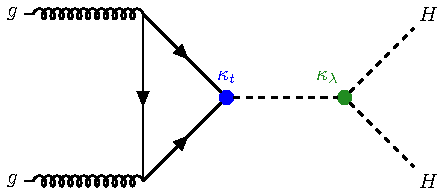
\includegraphics[width=0.45\textwidth]{figures/diHiggsSearches/fey_HH_Triangle.pdf} %
        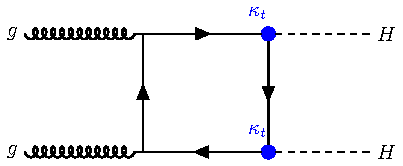
\includegraphics[width=0.45\textwidth]{figures/diHiggsSearches/fey_HH_Box.pdf}
    \end{center}
    \caption{Feynman diagrams for leading-order Higgs boson pair production via gluon fusion}
    \label{SMLO_ggHH_production}
\end{figure}
\begin{figure}[!htbp]
    \begin{center}
        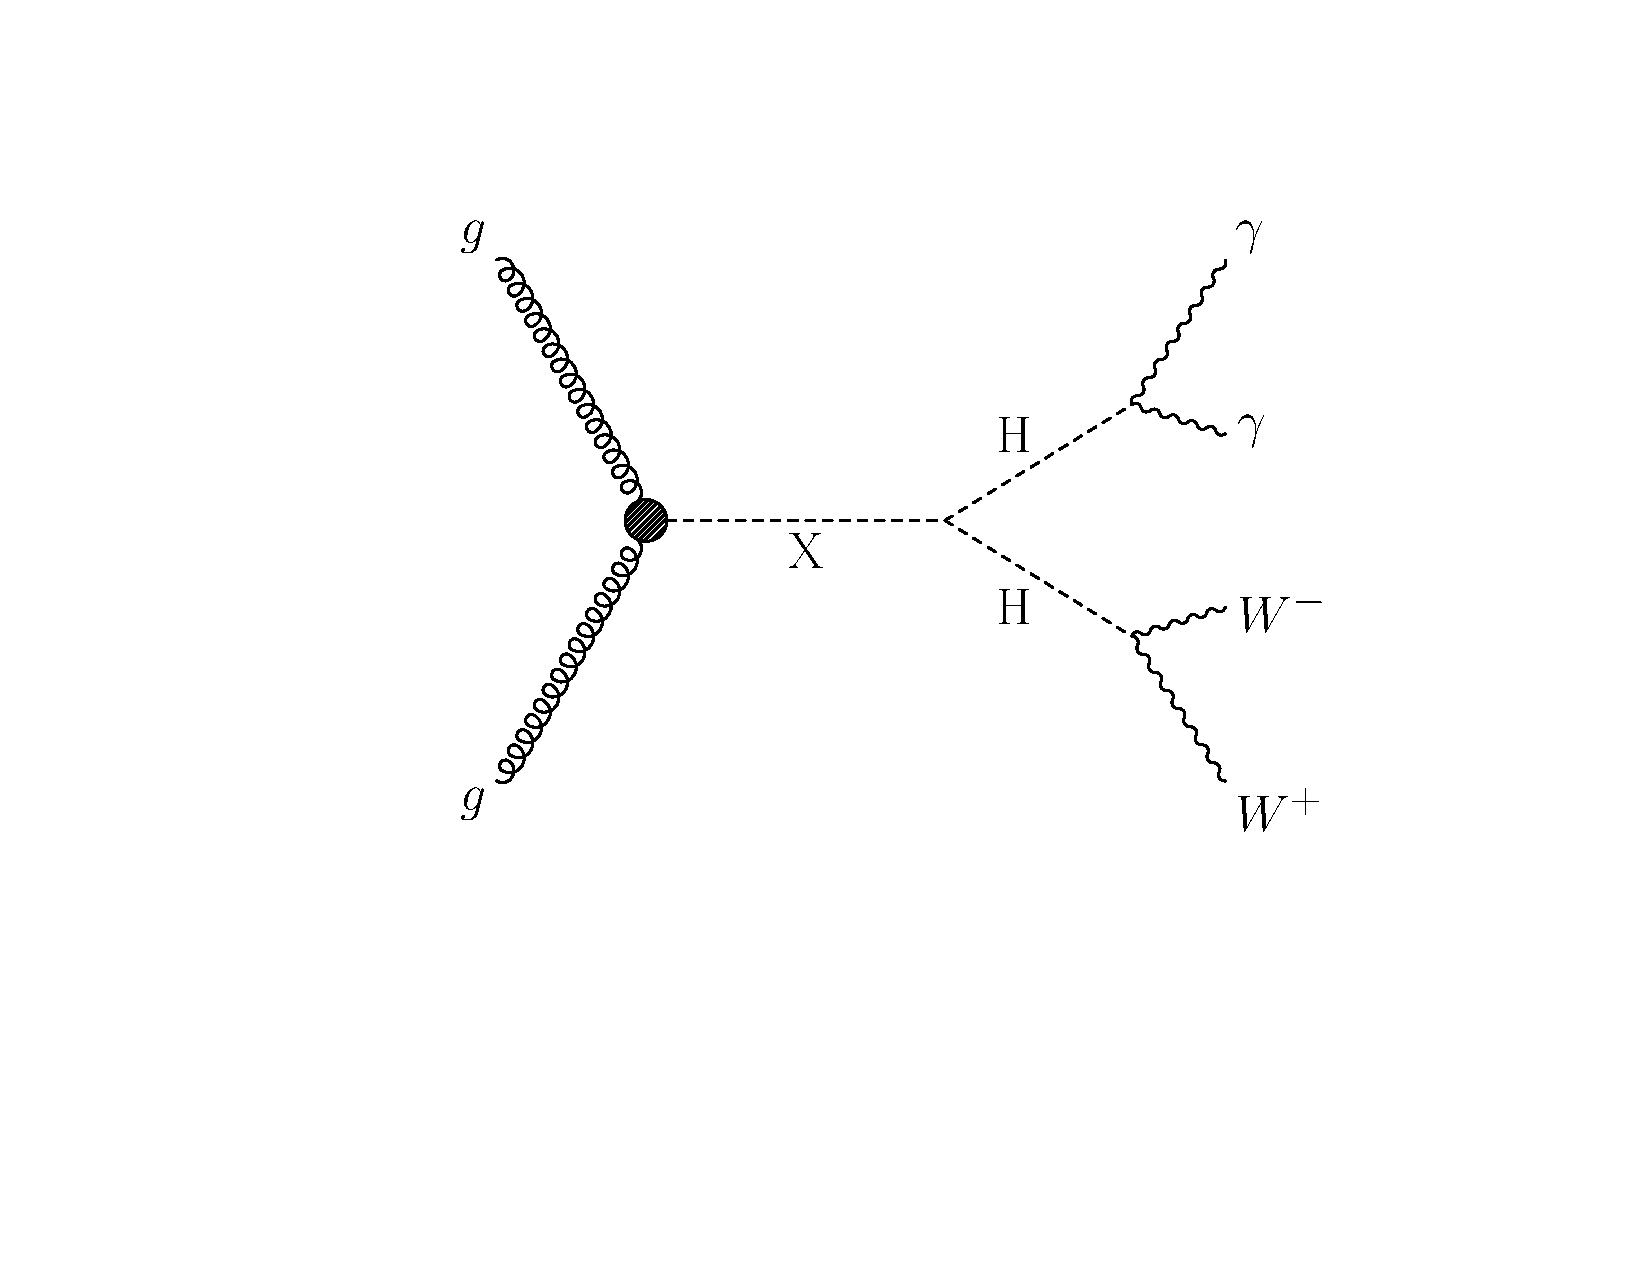
\includegraphics[width=0.45\textwidth]{figures/diHiggsSearches/fey_XHH_HHWWgg.pdf}
    \end{center}
    \caption{Feynman diagram for resonant di-Higgs production in the \HH channel}
    \label{XHHFeynmanDiagram}
\end{figure}


Extensions of the SM, such as the Next-to-Minimal Supersymmetric Standard Model (NMSSM), Randall-Sundrum models, or the two-Higgs
doublet model (2HDM), predict resonant di-Higgs production. In these scenarios, a heavy resonance \(X\) decays into two Higgs
bosons, which subsequently decay into \(WW\) and \(\gamma\gamma\), as shown in Fig.~\ref{XHHFeynmanDiagram}.

This analysis specifically targets the \(X \to HH \to WW\gamma\gamma\) channel, utilizing the clean diphoton final state to maximize sensitivity while accounting for all possible jet topologies.
Although this channel has a relatively low branching fraction, as shown in Fig.~\ref{fig:HH_BF},
it provides a distinctive signature for Beyond Standard Model (BSM) searches due to
the presence of a clean diphoton final state combined with couplings to vector bosons.

\begin{figure}[!htbp]
    \centering
    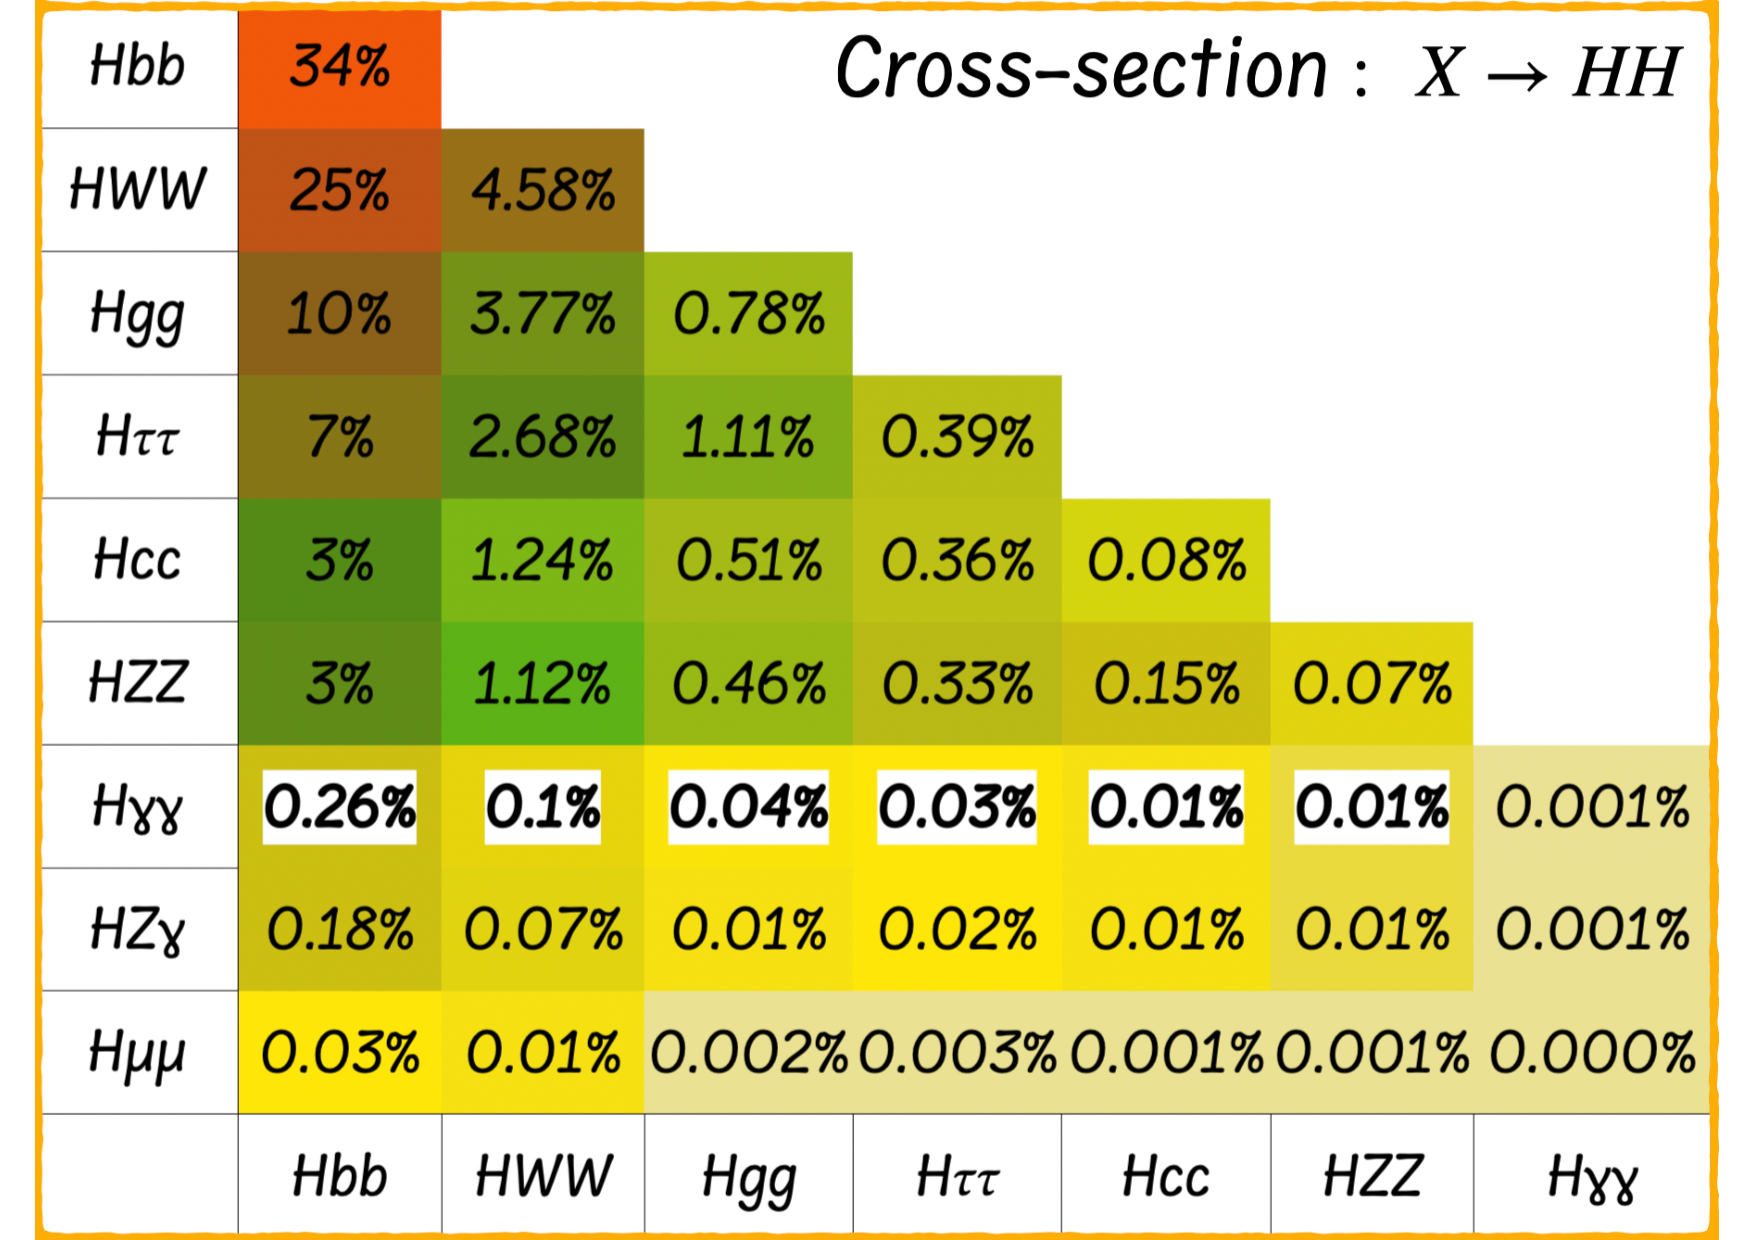
\includegraphics[width=0.95\textwidth]{figures/diHiggsSearches/HH_BF.pdf}
    \caption{Branching fractions of Higgs boson decays.}
    \label{fig:HH_BF}
\end{figure}


\section{Analysis Overview}
The analysis is performed using the full Run-2 Ultra-Legacy dataset, corresponding to an integrated luminosity of 138~fb\(^{-1}\) at
\(\sqrt{s} = 13\)~TeV. The following decay channels are explored:
\begin{itemize}
    \item \textbf{Semi-leptonic (\(l\nu qq\gamma\gamma\)):} One \(W\) boson decays leptonically (\(W \to l\nu\)), and the other
    decays hadronically (\(W \to qq\)).
    \item \textbf{Fully hadronic (\(4q\gamma\gamma\)):} Both \(W\) bosons decay hadronically (\(W \to qq\)).
\end{itemize}

\section{Unique Features of the Analysis}
This analysis incorporates several innovative aspects, as detailed below:

\begin{itemize}
    \item \textbf{Comprehensive Topology Coverage:}
    For the first time, all jet topologies are tagged within a single analysis. These include boosted, semi-boosted, resolved, and scenarios where leptons are reconstructed inside jets.

    \item \textbf{Signal Definition:}
    The signal is defined as the sum of three di-Higgs decay possibilities:
    \[
    HH \to WW\gamma\gamma + ZZ\gamma\gamma + bb\gamma\gamma.
    \]
    Since the hadronic decay topologies are similar for all three channels, it is challenging to reduce contamination from the \(ZZ\gamma\gamma\) and \(bb\gamma\gamma\) channels in our primary signal of interest, \(WW\gamma\gamma\). The signal definition is further refined with the following considerations:
    \begin{itemize}
        \item The analysis is optimized for the \(HH \to WW\gamma\gamma\) channel.
        \item For \(HH \to WW\gamma\gamma\), two decay modes of the \(W\)-bosons are considered: fully hadronic and semi-leptonic. The analysis optimization is performed based on these two final states.
        \item For \(HH \to ZZ\gamma\gamma\), due to the low branching fraction and negligible semi-leptonic contribution, the semi-leptonic decay mode is excluded from the analysis.
        \item The \(bb\gamma\gamma\) channel is included after applying a b-jet veto. This serves multiple purposes:
        \begin{enumerate}
            \item It reduces the contribution from the \(bb\gamma\gamma\) channel, ensuring that the limit is primarily driven by the \(WW\gamma\gamma\) channel rather than \(bb\gamma\gamma\).
            \item It makes the analysis orthogonal to the \(HH \to bb\gamma\gamma\) analysis.
            \item Events rejected by the \(HH \to bb\gamma\gamma\) analysis are exploited, thereby utilizing additional information from the same dataset.
            \item The b-jet veto also rejects events from \(HH \to ZZ\gamma\gamma\) where the \(Z\)-bosons decay into b-quarks.
        \end{enumerate}
    \end{itemize}

    \item \textbf{Mass Ranges:}
    The resonance \(X\) is studied over a mass range of 250~GeV to 3000~GeV.

    \item \textbf{Leptons Inside Jets:}
    Events where leptons are reconstructed within jets are included, thereby enhancing sensitivity to specific Beyond Standard Model (BSM) scenarios.
\end{itemize}

\section{Event Selection}


The event selection optimizes sensitivity to semi-leptonic and fully hadronic channels, with the following criteria:

\subsection*{Photon Selection}
\begin{itemize}
    \item A boosted decision tree (BDT) classifier is trained to separate photons from jets~\cite{Sirunyan:2018ouh}.
            The output of this BDT is referred to as the photon ID score
            \footnote{For the boosted regime, where the two photons are close by, the photon ID score was modified to
            account for reduced selection efficiency.
            This modified score is referred to as the ``modified photon ID," detailed in
            Appendix~\ref{appendix:ModifiedPhotonID}}. The photon $ID > -0.7$ is used as a preselection criterion.
    \item Leading photon \(p_T > 35\)~GeV and subleading photon \(p_T > 25\)~GeV.
    \item Photon transverse momentum fractions: \(p_T/m_{\gamma\gamma} > 0.33\) (leading) and \(> 0.25\) (subleading).
    \item Diphoton invariant mass requirement: \(100 < m_{\gamma\gamma} < 180\)~GeV.
\end{itemize}


\subsection*{Lepton Selection}
\begin{itemize}
    \item \textbf{Kinematics:} \(p_T > 10\)~GeV, \(|\eta| < 2.4\), and \(\Delta R(l, \gamma) > 0.4\).
    \item \textbf{\(Z\)-veto:} \(|m_{l\gamma} - 91.2| > 5\)~GeV to suppress contamination from \(Z\)-boson events.
    \item \textbf{ID requirements:}
        \begin{itemize}
            \item \textbf{For isolated electrons:} Use the isolated MVA ID with a signal efficiency of 80\%.
            \item \textbf{For isolated muons:} Require global muons with tight ID and an isolation threshold of 0.15.
            \item \textbf{For non-isolated electrons:} Use the non-isolated MVA ID with a signal efficiency of 80\%, ensuring \(\Delta R < 0.8\) with a good FatJet (as defined in the jet selection).
            \item \textbf{For non-isolated muons:} Require high \(p_T\) ID\todo[fancyline]{define High pT ID} without isolation criteria, ensuring \(\Delta R < 0.8\) with a good FatJet (as defined in the jet selection\todo[fancyline]{cite jet section}).
        \end{itemize}
\end{itemize}

\subsection*{Small Radius Jets (AK4 CHS)}
\begin{itemize}
    \item \textbf{ID:} Tight
    \item \textbf{PU Jet ID:} Tight
    \item \textbf{Kinematics:} \(p_T > 20\)~GeV, \(|\eta| < 2.4\)
    \item \textbf{Separation criteria:}
        \begin{itemize}
            \item \(\Delta R(\gamma, \text{jet}) > 0.4\)
            \item \(\Delta R(\text{Isolated Lepton, jet}) > 0.4\)
        \end{itemize}
\end{itemize}

\subsection*{FatJets (AK8 PUPPI)}
\begin{itemize}
    \item \textbf{Kinematics:} \(p_T > 100~\text{GeV}, |\eta| < 2.4\), with Tight Jet ID.
    \item \textbf{Separation criteria:}
    \begin{itemize}
        \item \(\Delta R(\gamma, \text{jet}) > 0.8\).
    \end{itemize}
    \item \textbf{Boosted \(H_{bb}\) jet veto:} \(X_{bb}/X_{\text{qcd}} < 0.9\).
    \item \textbf{Fully Hadronic Higgs Jet:}
    \begin{itemize}
        \item Particle Transformer\todo{define particle transformer in the footnote} Higgs Tagging score \(> 0.2\).
    \end{itemize}
    \item \textbf{Semi-Leptonic Higgs Jet:}
    \begin{itemize}
        \item \(\Delta R(\text{Non-isolated lepton}, \text{FatJet}) < 0.8\).
    \end{itemize}
    \item \textbf{Boosted \(W\)-Jet:}
    \begin{itemize}
        \item ParticleNet\todo{define particleNet in the footnote} loose working point for W-jet tagging.
        \item \(\Delta R(\text{Isolated leptons}, \text{FatJet}) > 0.8\).
    \end{itemize}
\end{itemize}

\subsection*{Event Selection}
The event selection is optimized for the semi-leptonic and fully hadronic channels and is summarized in Fig.~\ref{fig:event_selection_workflow}.
\begin{figure}[!htbp]
    \centering
    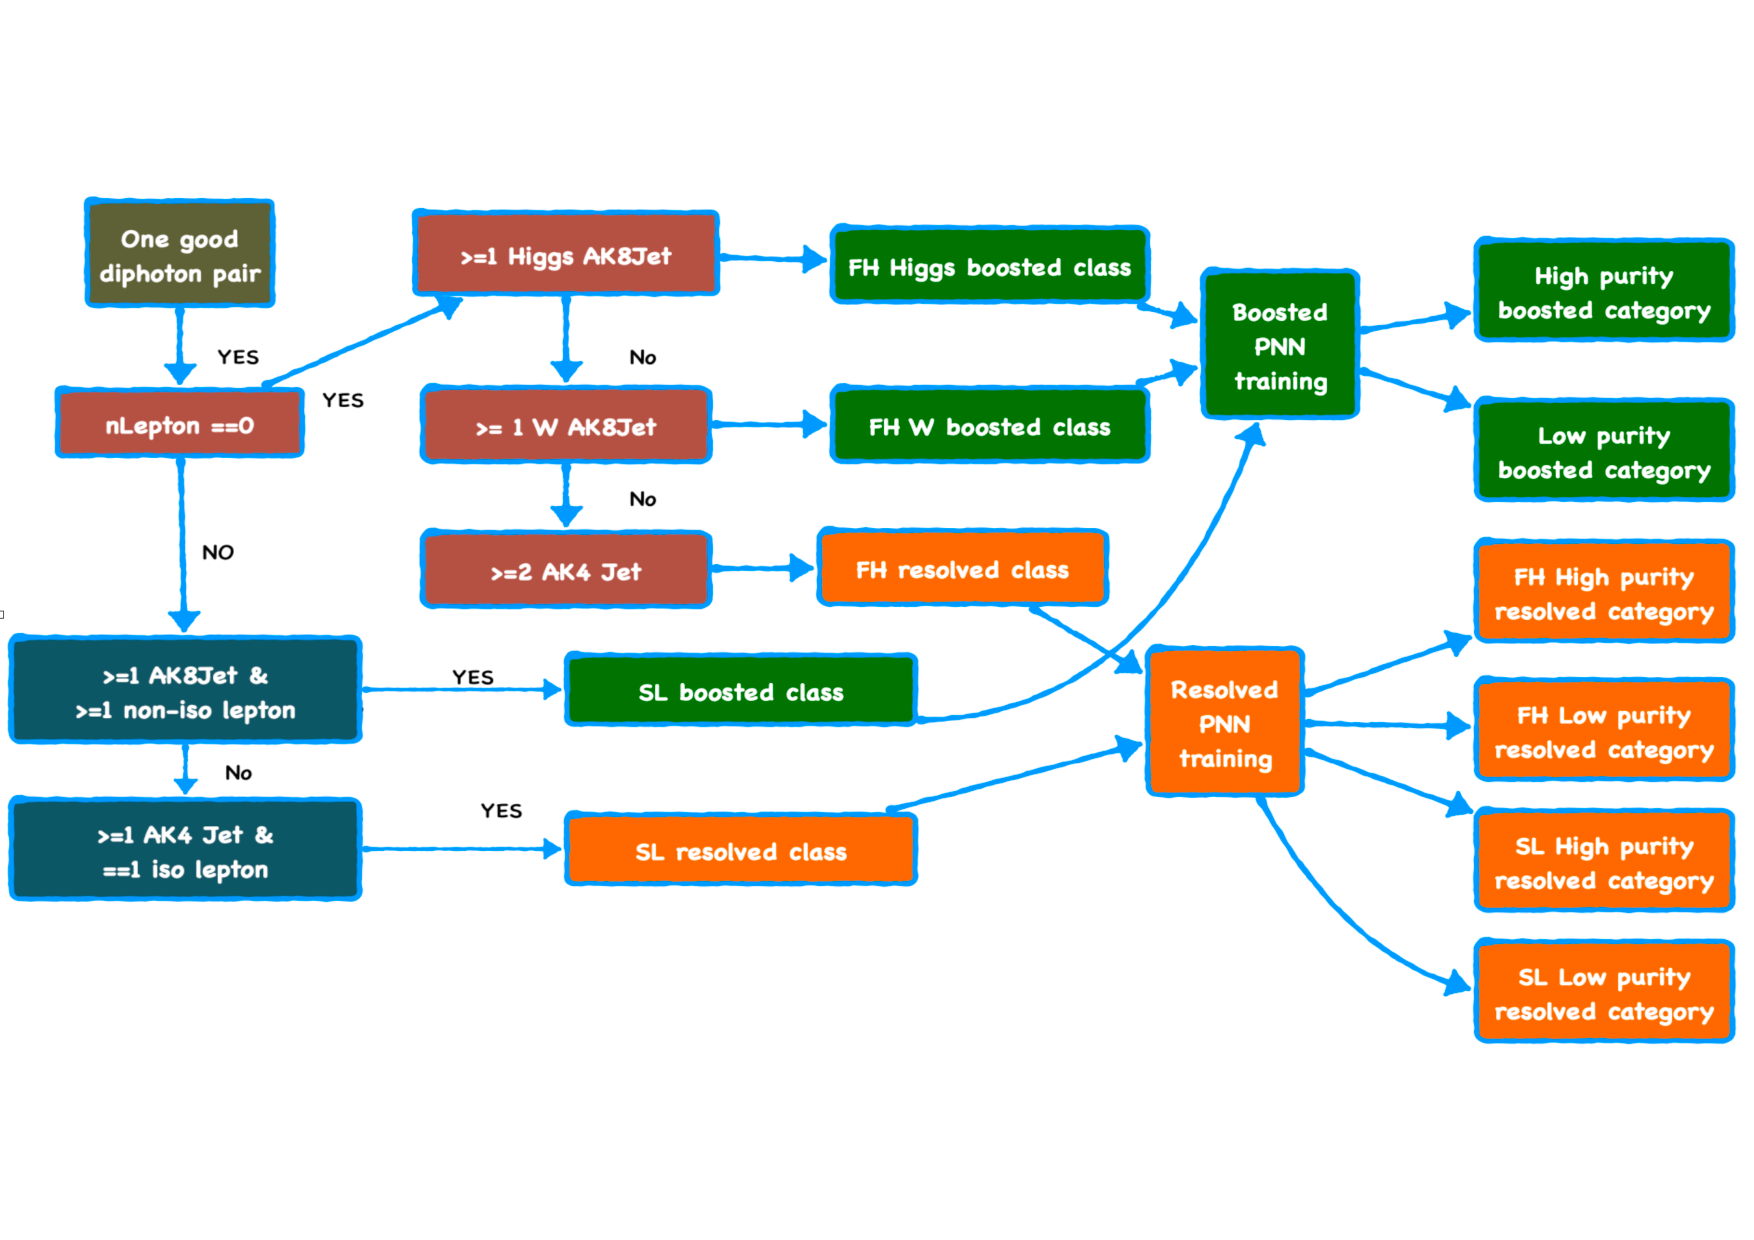
\includegraphics[width=0.95\textwidth]{figures/diHiggsSearches/EventSelectionWorkflow.pdf}
    \caption{Event selection workflow for the \(X \to HH \to WW\gamma\gamma\) analysis.}
    \label{fig:event_selection_workflow}
\end{figure}


\section{Data-Driven Background Estimation}
Accurately estimating background processes is crucial for isolating the \(X \to HH \to WW\gamma\gamma\) signal.
The dominant backgrounds include non-resonant diphoton production, single Higgs processes, and multijet events
where fake photons mimic the signal.
A data-driven approach is used to estimate fake photon contributions~\cite{CMS:2020cga}.

\subsection{Motivation}
The limited statistics of QCD Monte Carlo (MC) samples lead to poor modeling of key input features for multivariate analyses.
To ensure reliable machine learning training and data-MC agreement, a data-driven method is adopted~\cite{CMS:2020cga}.
This approach uses events from the photon ID MVA sideband to model fake photon contributions.

\subsection{Methodology}
The data-driven background estimation follows these steps:
\begin{enumerate}
    \item \textbf{Photon ID Sideband Selection:}
    Events failing the photon ID MVA preselection cut are used to model fake photons.
    The sideband regions are defined as:
    \begin{itemize}
        \item Resolved category: Photon ID MVA in \([-0.9, -0.7]\).
        \item Boosted category: Photon ID MVA in \([-0.95, -0.9]\).
    \end{itemize}

    \item \textbf{PDF Generation for Fake Photons:}
    A probability density function (PDF) for the photon ID MVA distribution of fake photons is
    derived from MC samples (e.g., \(\gamma + \text{jets}\)).
    Sideband events are reweighted to match the PDF in the signal region.

    \item \textbf{Reweighting and Normalization:}
    Per-event weights are applied to sideband events to reshape the photon ID MVA distribution.
    The weight \(w\) is defined as:
    \[
        w = \frac{\int_{\text{minID}}^{\text{maxID}} \text{fakePDF}(x) \, dx}
                 {\int_{\text{sidebandMinID}}^{\text{sidebandMaxID}} \text{fakePDF}(x) \, dx}.
    \]
    Separate weights are applied for resolved and boosted categories.

    \item \textbf{Validation:}
    The reweighted MC is normalized to data, and comparisons before and after reweighting show improved agreement in key variables like \(m_{\gamma\gamma}\).
\end{enumerate}

\subsection{Challenges and Solutions}
Despite its success, this method presents some challenges:
\begin{itemize}
    \item \textbf{Muon Channel in Semi-Leptonic (SL) Events:}
    While the method improves agreement in the electron channel, it worsens the muon channel.
    Potential solutions include:
    \begin{itemize}
        \item Applying the data-driven approach only to the electron channel.
        \item Using separate reweighting for electron and muon channels.
    \end{itemize}
    For now, we are using the additional MVA reweighting on top of this method to improve the overall agreement. As we don't use the MC for the signal extraction, the impact of this method on the signal extraction is minimal.

    \item \textbf{Photon ID Sidebands:}
    Key assumptions in this method include:
    \begin{enumerate}
        \item Photon ID MVA has minimal correlation with other analysis variables.
        \item The sideband is dominated by fake photons (e.g., QCD and \(\gamma + \text{jets}\)).
        \item Sideband photons are assumed to be entirely fake.
    \end{enumerate}
\end{itemize}

\subsection{Implementation in Different Channels}
The method is applied to both fully hadronic (FH) and semi-leptonic (SL) channels:
\begin{itemize}
    \item \textbf{Fully Hadronic Channel:}
    Dominated by QCD backgrounds, with the photon ID sideband effectively modeling fake photon contributions.
    \item \textbf{Semi-Leptonic Channel:}
    Includes contributions from \(W\gamma\gamma\) and \(t\bar{t}\) processes, with non-isolated leptons playing a key role in background estimation.
\end{itemize}

\subsection{Impact of the Data-Driven Method}
The data-driven background estimation significantly improves the analysis:
\begin{itemize}
    \item Enhanced modeling of photon-related variables in resolved and boosted categories.
    \item Improved agreement between data and MC in control regions, as shown in Fig.~\ref{fig:control_plots}.
    \missingfigure{control plots}\label{fig:control_plots}
\end{itemize}

\section{Multivariate Analysis Using Parameterized Neural Network (pNN)}

To maximize the sensitivity of the search for resonant \(X \to HH \to WW\gamma\gamma\), a multivariate analysis (MVA) is performed
using a Parameterized Neural Network (pNN). The pNN method allows for simultaneous training across multiple signal hypotheses,
parameterized by the mass of the heavy resonance \(m_X\). This approach ensures a robust discrimination between signal and
background across a wide range of masses, from 250~GeV to 3000~GeV.

The pNN is implemented as a deep feed-forward neural network. Its inputs include kinematic and topological features of the events, with the resonance mass \(m_X\) incorporated as a parameter to generalize across different signal hypotheses. The network is trained using the Adam optimizer with stochastic gradient descent, and GPU acceleration is used for efficient processing of large datasets. Additional features, such as dropout layers, are included to prevent overfitting and enhance model generalization.

Separate pNNs are trained for the boosted and resolved topologies to account for the distinct event kinematics in these categories.
The boosted category includes events where \(W\)-bosons' decay products are merged into single AK8 jets, while the resolved category reconstructs \(W\)-bosons' decay products as individual AK4 jets.
Input features, such as photon, jet, and missing transverse energy (\(E_T^{\text{miss}}\)) observables, are carefully selected based on their ability to discriminate signal from background. These features include variables like the diphoton \(p_T/m_{\gamma\gamma}\), the angular separation (\(dR\)) between photons, and jet kinematics. The full list of input variables used for the boosted pNN training is provided in Table~\ref{tab:inputvariables_boosted} and for the resolved pNN training in Table~\ref{tab:inputvariables_resolved}.
\begin{table}[htbp!]
    \centering
    \begin{tabularx}{\textwidth}{|l|X|}
    \hline
    \textbf{Feature} & \textbf{Description} \\
    \hline
    Diphoton\_pTom & Transverse momentum of the diphoton system over the mass of the diphoton system \\
    Diphoton\_dR & Delta R between the two photons \\
    Diphoton\_eta & Pseudorapidity of the diphoton system \\
    Diphoton\_phi & Azimuthal angle of the diphoton system \\
    LeadPhoton\_pTom & Transverse momentum of the leading photon over the mass of the diphoton system \\
    SubleadPhoton\_pTom & Transverse momentum of the subleading photon over the mass of the diphoton system \\
    LeadPhoton\_eta & Pseudorapidity of the leading photon \\
    LeadPhoton\_phi & Azimuthal angle of the leading photon \\
    SubleadPhoton\_eta & Pseudorapidity of the subleading photon \\
    SubleadPhoton\_phi & Azimuthal angle of the subleading photon \\
    fatjet\_1\_pT & Transverse momentum of the leading fatjet \\
    fatjet\_1\_eta & Pseudorapidity of the leading fatjet \\
    fatjet\_1\_phi & Azimuthal angle of the leading fatjet \\
    fatjet\_1\_mass & Mass of the leading fatjet \\
    fatjet\_2\_pT & Transverse momentum of the subleading fatjet \\
    fatjet\_2\_eta & Pseudorapidity of the subleading fatjet \\
    fatjet\_2\_phi & Azimuthal angle of the subleading fatjet \\
    fatjet\_2\_mass & Mass of the subleading fatjet \\
    fatjet\_1\_2\_dR & Delta R between the two fatjets \\
    fatjet\_1\_diphoton\_dR & Delta R between the leading fatjet and the diphoton system \\
    fatjet\_2\_diphoton\_dR & Delta R between the subleading fatjet and the diphoton system \\
    fatjet\_1\_leadphoton\_dR & Delta R between the leading fatjet and the leading photon \\
    fatjet\_1\_subleadphoton\_dR & Delta R between the leading fatjet and the subleading photon \\
    fatjet\_2\_leadphoton\_dR & Delta R between the subleading fatjet and the leading photon \\
    fatjet\_2\_subleadphoton\_dR & Delta R between the subleading fatjet and the subleading photon \\
    max\_fatjets\_mass & Maximum mass of the two fatjets \\
    nGoodAK4jets & Number of good AK4 jets \\
    nGoodAK8jets & Number of good AK8 jets \\
    Third leading jets\_pT & Transverse momentum of the third leading jets \\
    Third leading jets\_eta & Pseudorapidity of the third leading jets \\
    Third leading jets\_phi & Azimuthal angle of the third leading jets \\
    Third leading jets\_mass & Mass of the third leading jets \\
    PuppiMET\_pt & Transverse momentum of the missing transverse energy \\
    dphi\_jet1\_PuppiMET & Azimuthal angle difference between the first jet and missing transverse energy \\
    dphi\_jet2\_PuppiMET & Azimuthal angle difference between the second jet and missing transverse energy \\
    PuppiMET\_sumEt & Sum of the transverse energy of the missing transverse energy \\
    MX & Invariant mass of the resonance X \\
    \hline
    \end{tabularx}
    \caption{Input variables used for the boosted PNN training.}
    \label{tab:inputvariables_boosted}
\end{table}
\begin{table}[htbp!]
    \centering
    \begin{tabularx}{\textwidth}{|l|X|}
    \hline
    \textbf{Feature} & \textbf{Description} \\
    \hline
    MX & Invariant mass of the resonance X \\
    Diphoton\_pTom & Transverse momentum of the diphoton system over the mass of the diphoton system \\
    Diphoton\_eta & Pseudorapidity of the diphoton system \\
    Diphoton\_phi & Azimuthal angle of the diphoton system \\
    LeadPhoton\_pTom & Transverse momentum of the leading photon over the mass of the diphoton system \\
    SubleadPhoton\_pTom & Transverse momentum of the subleading photon over the mass of the diphoton system \\
    LeadPhoton\_eta & Pseudorapidity of the leading photon \\
    LeadPhoton\_phi & Azimuthal angle of the leading photon \\
    SubleadPhoton\_eta & Pseudorapidity of the subleading photon \\
    SubleadPhoton\_phi & Azimuthal angle of the subleading photon \\
    Diphoton\_dR & Delta R between the two photons \\
    Diphoton\_dEta & Delta pseudorapidity between the two photons \\
    jet\_1\_2\_pt & Transverse momentum of the combined leading and subleading jets \\
    jet\_1\_2\_mass & Mass of the combined leading and subleading jets \\
    jet\_1\_2\_dR & Delta R between the leading and subleading jets \\
    jet\_1\_pt & Transverse momentum of the leading jet \\
    jet\_2\_pt & Transverse momentum of the subleading jet \\
    photon1\_jet1\_dR & Delta R between the leading photon and the leading jet \\
    photon1\_jet2\_dR & Delta R between the leading photon and the subleading jet \\
    photon1\_jet1\_2\_dR & Delta R between the leading photon and the combined leading and subleading jets \\
    Diphoton\_jet1\_2\_dR & Delta R between the diphoton system and the combined leading and subleading jets \\
    Diphoton\_jet1\_dR & Delta R between the diphoton system and the leading jet \\
    Diphoton\_jet2\_dR & Delta R between the diphoton system and the subleading jet \\
    photon2\_jet1\_dR & Delta R between the subleading photon and the leading jet \\
    photon2\_jet2\_dR & Delta R between the subleading photon and the subleading jet \\
    photon2\_jet1\_2\_dR & Delta R between the subleading photon and the combined leading and subleading jets \\
    Diphoton\_jet\_1\_2\_dEta & Delta pseudorapidity between the diphoton system and the combined leading and subleading jets \\
    Diphoton\_jet\_1\_dEta & Delta pseudorapidity between the diphoton system and the leading jet \\
    Diphoton\_jet\_2\_dEta & Delta pseudorapidity between the diphoton system and the subleading jet \\
    Diphoton\_jet\_1\_2\_dPhi & Delta phi between the diphoton system and the combined leading and subleading jets \\
    Diphoton\_jet\_1\_dPhi & Delta phi between the diphoton system and the leading jet \\
    Diphoton\_jet\_2\_dPhi & Delta phi between the diphoton system and the subleading jet \\
    PuppiMET\_pt & Transverse momentum of the missing transverse energy \\
    nGoodAK4jets & Number of good AK4 jets \\
    nGoodisoleptons & Number of good isolated leptons \\
    leading\_bscore & B-tagging score of the leading jet \\
    subleading\_bscore & B-tagging score of the subleading jet \\
    sum\_two\_max\_bscores & Sum of the two highest b-tagging scores \\

    \hline
    \end{tabularx}
    \caption{Input variables used for the resolved PNN training.}
    \label{tab:inputvariables_resolved}
\end{table}

The performance of the pNN is evaluated using metrics such as the area under the curve (AUC) and signal-to-background ratio improvements. The pNN demonstrates significant enhancement in discrimination between signal and background across the entire mass range. Feature importance plots highlight the critical role of variables such as diphoton \(p_T/m_{\gamma\gamma}\) and photon angular separations in improving sensitivity. Separate training for the boosted and resolved categories further optimizes the analysis for these topologies.

The output of the pNN serves as the final discriminant for signal extraction in the \(m_{\gamma\gamma}\) distribution. By combining the boosted and resolved categories, the analysis achieves a 60\% improvement in sensitivity compared to previous results. Control plots of key variables before and after applying the pNN show excellent agreement between data and Monte Carlo, validating the robustness of the method.

The parameterized neural network approach thus provides a powerful framework for signal extraction in the \(X \to HH \to WW\gamma\gamma\) analysis. By training across multiple mass hypotheses and incorporating advanced multivariate techniques, the pNN significantly improves the sensitivity to resonant di-Higgs production, particularly in high-mass regions.

\section{Systematic uncertainties}
\label{section:Systematics}
The systematic uncertainties detailed below are taken into account in the statistical model via profiling of nuisance parameters according to a frequentist approach.
Effect from several sources are considered, including theoretical uncertainties, experimental uncertainties, and uncertainties in the background modeling.

Most systematic uncertainties are represented by log-normal probability distribution functions, which parameterize the event yield in each signal region. These uncertainties impact the overall normalization of the signal and resonant background processes in each signal region (and can vary by region) but do not affect the shape of the \mgg distribution.

The second type of systematic uncertainty affects the shape (and potentially the normalization) of the \mgg distributions for both signal and resonant background processes, as well as the non-resonant background modeled from data. These uncertainties are incorporated as nuisance parameters in the signal models for each signal region.
Specifically, the uncertainty related to the choice of function for background modeling is handled as a discrete nuisance parameter, using the discrete profiling method~\cite{Dauncey:2014xga}.

The different sources of uncertainties and their ranges are summarized in Table~\ref{table:sys-tab}.
  \begin{table}[!htbp]
    \begin{center}
    \resizebox*{1\textwidth}{!}{
    \begin{tabular}{l | c | c | c | c | c | c}
    \hline
    Source & Correlation(2017/2018) & Category(FH/SL,Resolved/Boosted) &  Type & Effect in WW$\gamma\gamma$ & Effect in bb$\gamma\gamma$ & Effect in ZZ$\gamma\gamma$\\ \hline
    \hline

    % AlphaS & lnN & - & - & - \\
    Branching ratio $H\rightarrow \gamma\gamma$ & Correlated & All & lnN &  0.9874/1.0214 & 0.9874/1.0214 & 0.9874/1.0214 \\
    Branching ratio $H\rightarrow WW$ &  Correlated & All & lnN &  0.9848/1.0153 & - & - \\
    Branching ratio $H\rightarrow bb$ &  Correlated & All & lnN &  - & 0.9874/1.0124 & - \\
    Branching ratio $H\rightarrow ZZ$ &  Correlated & All & lnN &  - & - & 0.9848/1.0153 \\
    % Parton shower & shape & - & - & - \\
    % \textcolor{red}{QCD scale acceptance} & shape & - & - & - \\
    % \textcolor{red}{PDF acceptance} & shape & - & - & - \\

    \hline

    Luminosity & Uncorrelated & All & lnN & 1.010-1.020 & 1.010-1.020 & 1.010-1.020 \\
    Luminosity & Correlated & All & lnN & 1.006-1.020 & 1.006-1.020 & 1.006-1.020 \\
    Photon Trigger & Uncorrelated & All & lnN & 1.0021 & 1.0021 & 1.0021 \\
    Photon Energy Scaling & Uncorrelated & All & shape & \checkmark & \checkmark & \checkmark \\
    Photon Energy Resolution & Uncorrelated & All & shape & \checkmark & \checkmark & \checkmark \\
    ECAL Material & Correlated & All & shape & \checkmark & \checkmark & \checkmark \\
    FNUF  & Correlated & All & shape &  \checkmark & \checkmark & \checkmark \\
    L1 Pre-fire & Uncorrelated & All & lnN & 0.988-0.999 & 0.989-0.999 & 0.99-0.999 \\
    Pileup & Uncorrelated & All &  lnN & 0.994-1.001 & 0.981-1.019 & 0.992-1.012 \\
    % \textcolor{red}{Pileup Jet ID} & Correlated & All & lnN & \textcolor{red}{-}  & \textcolor{red}{-} & \textcolor{red}{-} \\
    {Pileup Jet ID} & Correlated & All & lnN & 0.928-1.076  & 0.948,1.064 & 0.98-1.021 \\
    \hline
    {b-tag lf/hf stats} & Uncorrelated & FH Resolved & lnN & 0.928-1.28  & 0.903-1.357 & 0.931-1.312 \\
    {b-tag JES} & Correlated & FH Resolved & lnN & 0.962-1.025  & 0.958-1.036 & 0.962-1.031 \\
    {b-tag Purity} & Correlated & FH Resolved & lnN &  0.952-1.261  & 0.919-1.431 & 0.961-1.215 \\
    {b-tag Charm Jets} & Correlated & FH Resolved & lnN & 0.805-1.256  & 0.762-1.431 & 0.821-1.218 \\
    \hline
    Electron-veto SF & Uncorrelated & SL All & lnN & 1.001-1.003 & 1.001-1.002 & 1.001-1.003 \\
    Electron Reconstruction & Uncorrelated & SL All & lnN & 0.952-1.048 & 0.983-1.026 & 0.952-1.046 \\
    Electron Identification & Uncorrelated & SL All & lnN & 1.001-1.008 & 1.001-1.007 & 1.006-1.013 \\
    Muon Identification & Uncorrelated & SL All & lnN & 1.001-1.003 & 1.002 & 1.002-1.003 \\
    Muon Isolation & Uncorrelated & SL All & lnN & 1.001-1.003 & 1.002 & 1.002-1.003 \\
    DiPhoton Preselection SF & Uncorrelated & All & lnN & 0.954-1.047 & 0.954-1.047 & 0.954-1.047 \\
    Photon Identification & Uncorrelated & All & lnN & 0.957-1.044 & 0.952-1.049 & 0.956-1.044 \\
    \hline
    JEC  &  Uncorrelated & All & lnN & 0.875-1.156 & 0.834-1.166 & 0.882-1.105 \\
    % JEC Absolute\_YEAR  &  Uncorrelated & All & lnN & 0.997-1.006 & 0.997-1.003 & 0.998-1.005 \\
    % JEC BBEC1  &  Correlated & All & lnN & 0.997-1.006 & 0.997-1.003 & 0.998-1.005 \\
    % JEC BBEC1\_YEAR  &  Uncorrelated & All & lnN & 0.997-1.006 & 0.997-1.003 & 0.998-1.005 \\
    % JEC EC2  &  Correlated & All & lnN & 0.997-1.006 & 0.997-1.003 & 0.998-1.005 \\
    % JEC EC2\_YEAR  &  Uncorrelated & All & lnN & 0.997-1.006 & 0.997-1.003 & 0.998-1.005 \\
    % JEC HF  &  Correlated & All & lnN & 0.997-1.006 & 0.997-1.003 & 0.998-1.005 \\
    % JEC HF\_YEAR  &  Uncorrelated & All & lnN & 0.997-1.006 & 0.997-1.003 & 0.998-1.005 \\
    % JEC RelativeBal  &  Correlated & All & lnN & 0.997-1.006 & 0.997-1.003 & 0.998-1.005 \\
    % JEC RelativeSample\_YEAR  &  Uncorrelated & All & lnN & 0.997-1.006 & 0.997-1.003 & 0.998-1.005 \\
    % JEC FlavorQCD  &  Correlated & All & lnN & 0.997-1.006 & 0.997-1.003 & 0.998-1.005 \\
    \hline
    JER & Uncorrelated & All & lnN & 1.001-1.002 & 1.001-1.003 & 1.001 \\
    MET Unclustered Energy & Uncorrelated & All &  lnN & - & - & - \\
    Muon Momentum Rochester Correction & Uncorrelated & SL All  & lnN & - & 1.001-1.002 & - \\
    PNet bb-tag efficiency & Uncorrelated & FH Boosted  &  lnN & - & 0.77-1.472 & -\\
    % \textcolor{red}{PNet bb-tag efficiency} & Uncorrelated & FH Boosted  &  lnN & - & 0.77-1.472 & -\\
    PNet WvsQCD efficiency & Uncorrelated & FH Boosted & lnN & 0.995-1.005  & 0.992-1.009 & 0.987-1.013 \\
    ParT HvsQCD efficiency & Uncorrelated & FH Boosted & lnN & 0.775-1.198 & 0.829-1.151 & 0.768-1.204 \\

    \hline
    \hline
    \end{tabular}
    }
    % \caption{Summary of systematic uncertainties (top: theoretical, bottom: experimental). Uncertainties in \textcolor{red}{red} are not yet implemented in the datacards.}
    \caption{Summary of systematic uncertainties (top: theoretical, bottom: experimental).}
    \label{table:sys-tab}
    \end{center}
  \end{table}

  \subsection{Theoretical uncertainties}
The theory uncertainties can affect the normalization of both the signal processes and the background single higgs processes.
\begin{itemize}
    \item \textbf{parton density functions (PDF) uncertainties}: The combined uncertainty on the parton density functions (PDF) is directly adapted from ~\cite{CMS:gghhrecommendations} where the size of these uncertainties is less than 3\%. Only single Higgs production is considered to add the PDF uncertainties.
\end{itemize}
\begin{itemize}
      \item \textbf{QCD scale variation} This variation is related to the uncertainty of the QCD renormalization and factorization scales. As a theoretical uncertainty it is also fully correlated among years and analysis bins. The migration uncertainty between analysis bins caused by the QCD scales are estimated by varying both scales by a factor of 2 in the same direction simultaneously. Only single Higgs production is considered to add the QCD scale uncertainties.
  \end{itemize}
\begin{itemize}
      \item \textbf{\alpS uncertainy} This uncertainty is related to the variation of the value of the strong force coupling constant. As the PDF uncertainty it is taken from the \textsc{pdf4lhc} prescription. It is evaluated in the same way as the QCD scale uncertainty by varying \alpS instead of the scales. Only single Higgs production is considered to add the \alpS uncertainties.
  \end{itemize}
  \begin{itemize}
      \item \textbf{$H \rightarrow \gamma\gamma$ branching fraction}: Values are taken from Ref.~\cite{florian2016handbook} and are estimated to be around 2\%.
      \item \textbf{$H \rightarrow WW$ branching fraction}: Values are taken from Ref.~\cite{run2HHcombination} and are estimated to be around 1.5\%.
      \item \textbf{$H \rightarrow ZZ$ branching fraction}: Values are taken from Ref.~\cite{run2HHcombination} and are estimated to be around 1.5\%.
      \item \textbf{$H \rightarrow bb$ branching fraction}: Values are taken from Ref.~\cite{run2HHcombination} and are estimated to be around 1.2\%.
  \end{itemize}

\subsection{Experimental uncertainties}
Here we describe the sources of experimental uncertainty.
Experimental uncertainties may either affect the shape and normalization of the \mgg distribution or simply the normalization.

Those affecting the shape of the \mgg distribution include:
\begin{itemize}
    \item \textbf{Photon energy scale and resolution} This is the uncertainty related to the scale of the photon energy in data and its smearing correction \cite{Scales_AN} in simulation. The variations are evaluated using Zee events by varying the energy regression training scheme, the \RNINE~ distribution, and the selection criteria. The scale uncertainty amounts to $0.05$ to $0.15$ \% for most of the photons, while they can go up to $3$ \% for some.
    Note that the scales and smearings applied by default in nanoAOD have been validated in the EGM and XPOG groups taken from the following presentations:
\begin{itemize}
    \item \href{https://indico.cern.ch/event/1123547/contributions/4716514/attachments/2394644/4097503/CrossPOG_23Feb2022.pdf}{\textcolor{blue}{\underline{XPOG 23 Feb 2022}}}
    \item \href{https://indico.cern.ch/event/1095390/contributions/4799715/attachments/2421381/4144630/CMSweek_5Apr2022.pdf}{\textcolor{blue}{\underline{CMS Week 5 Apr 2022}}}
\end{itemize}
The sytematics are added to the v9 nanoAOD produced centrally. The branches used are the dESigma up and down variations refer from CMSSW \cite{CMSSW_smear}.
  \end{itemize}

% \begin{itemize}
%     \item \textbf{Photon energy resolution}: the uncertainty associated with the corrections derived to match the photon energy resolution in simulation with that observed in data. The sytematics are added to the v9 nanoAOD produced centrally. The branches used are the dESigma up and down variations - \href{https://github.com/cms-sw/cmssw/blob/master/PhysicsTools/NanoAOD/python/photons_cff.py#L326-L327}{\textcolor{blue}{\underline{CMSSW reference}}}.
% \end{itemize}
\begin{itemize}
    \item \textbf{Modelling of the material upstream of ECAL} The showering behaveiour of photons is influenced by the material that is in front of ECAL. This systematic variation is associated to the uncertainty in these models. Its impact on the photon energy scale is evaluated by varying the amount of upstream material in the simulation. It amounts to $0.02$ to $0.05$ \% for central photons and goes up to $0.25$ \% for photons in the endcap.
\end{itemize}
\begin{itemize}
    \item \textbf{FNUF uncertainty}: differences in light collection efficiency (LCE) along the length of ECAL crystals result in different responses to electrons and photons. The uncertainty is estimated using the LCE model described in~\cite{Adams:2016viv}, derived from optical simulation~\cite{Gentit:2001ky}.
\end{itemize}

% Note that the scales and smearings applied by default in nanoAOD have been validated in the EGM and XPOG groups, as shown by the plots in Fig.~\ref{fig:syst_zee} taken from the following presentations:
% \begin{itemize}
%     \item \href{https://indico.cern.ch/event/1123547/contributions/4716514/attachments/2394644/4097503/CrossPOG_23Feb2022.pdf}{\textcolor{blue}{\underline{XPOG 23 Feb 2022}}}
%     \item \href{https://indico.cern.ch/event/1095390/contributions/4799715/attachments/2421381/4144630/CMSweek_5Apr2022.pdf}{\textcolor{blue}{\underline{CMS Week 5 Apr 2022}}}
% \end{itemize}

Experimental uncertainties affecting only the normalization of a given process include:
\begin{itemize}
    \item \textbf{Integrated luminosity}: An estimated uncorrelated uncertainty of 1.5\% for 2018, 2\% for 2017 and 1\% for 2016 is used  as recommended by the LUMI POG ~\cite{CMS-LUM-17-003,CMS-PAS-LUM-17-004,CMS-PAS-LUM-18-002}. Correlated uncertainties between 2017(0.6\%) and 2018(0.2\%), between 2016(0.6\%), 2017(0.9\%) and 2018(2\%) are used as recommended by the LUMI POG ~\cite{CMS:LUMI}.
    \item \textbf{L1 prefiring}: the inefficiency due to the prefiring of the L1 trigger during 2016 and 2017 data-taking periods is estimated following the recommended treatment from the JetMET group~\footnote{https://twiki.cern.ch/twiki/bin/viewauth/CMS/L1ECALPrefiringWeightRecipe}. The uncertainty is taken as the maximum between 20\% of the object prefiring probability and the statistical uncertainty associated to the considered bin in the prefiring map. The prefiring central weight and up/down variations are computed using the recipe in \href{https://github.com/cms-nanoAOD/nanoAOD-tools}{\textcolor{blue}{\underline{nanoAOD tools}}}. The corresponding uncertainties on signal efficiency is found to be up to 0.4\%
    \item \textbf{Trigger}: the trigger efficiency is measured from $Z \to ee$ events using the tag-and-probe technique; the size of the uncertainty varies between the photon categories, which are binned in $R_9$, $\eta$ and $p_T$. Typical values are well below the 1\% level and result in event yield variations of at most 0.1\%.
    \item \textbf{PU weighting}: the pu central reweighting and up/down variations are computed usign the recipe in \href{https://github.com/cms-nanoAOD/nanoAOD-tools}{\textcolor{blue}{\underline{nanoAOD tools}}}.
	\item \textbf{Diphoton preselection scale factors}: the uncertainty in the diphoton preselection efficiency is estimated from the ratio of the efficiency as calculated in data versus that calculated in simulation. The corresponding uncertainties on signal efficiency is found to be up to 4.7\% referring to ~\cite{AN-21-025}.
	\item \textbf{Photon ID MVA scale factors}: The corrections to the modified photonID MVA have been approved by EGammaPOG~\cite{CMS:Egammameetingmodifiedmvasf} and are implemented in the MC samples. The corresponding uncertainties on signal efficiency is found to be around 3\%
	\item \textbf{Electron Veto scale factors}: similar to the pixel seed veto uncertainty, the uncertainty in the scale factors applied to simulation to match the efficiency of the electron veto, derived using Z $\to \mu\mu$ + $\gamma$ events.
	\item \textbf{Electron ID and ISO scale factors}: Following the EGamma POG UL Run2 recommendation \cite{CMS:electron}, the corrections of the electron ID with isolation are applied to simulation. The corresponding uncertainties on signal efficiency is found to be up to 1.2\%.
  \item \textbf{Muon ID and ISO scale factors}: Following the Muon POG recommendation \cite{CMS:muon}, we use scale factors and uncertainties provided for muon ID, isolation, reconstruction efficiency. MC events are reweighted as a function of the muon $\pt$ and $\eta$, except for the muon reconstruction scale factors which are provided as a function of the muon $p$ and $\eta$. The corresponding uncertainties are obtained by varying each scale factor independently by $\pm 1 \sigma$. Tight ID and Tight ISO corrections are applied to isolated muon simulation events, Highpt ID and reconstruction corrections are applied to non-isolated muon simulation events. %FIXME: The reconstruction sf is not applied to isolated muons, but the ID and ISO are.
  \item \textbf{Shape of the DeepJet b-tag discriminant}:To correct the shape of DeepJet discriminant coming from simulation to match with data, reshaping scale factors are used, depending on \pt, $\eta$ and flavor of the jets.The uncertainty associated with this SFs measurement is obtained by comparing b discriminator distribution between data and simulation.
  \item \textbf{PUJetID}: Following the JetMET POG recommendation \cite{pileupid}, we use scale factors and uncertainties provided by JetMET POG \cite{JMEjsonpog}for tight PUJetID.

  \item \textbf{Jet Energy scale and resolution}: the JES global up and down variations and the JER variations are used to compute the Jet
  momentum systematic uncertainties. The MET is affected by the same systematics. Additionally, an uncertainty source sue to the MET
  unclustered component is considered. The uncertainties are applied using the NanoAOD Tools module \href{https://github.com/shaoweisong/NanoAODTools/blob/HHWWgg/python/postprocessing/modules/jme/jetmetHelperRun2.py}{\textcolor{blue}{\underline{nanoAOD tools}}}. The latest available JES and JER tags derived by the Jet-MET Group \cite{CMS:JER} for AK8 PUPPI and AK4 CHS Jets are used.%namely:
  \item \textbf{Muon Rochester \( p_T \) corrections}: the latest available muon rochester corrections for run2.v5 are used for the muon scale as recommended by the MUON POG \cite{CMS:muonrocch}. The relative up and down uncertainties are applied. %(do we want rochester muon corrections or muon POG pT is ok?)

  \item \textbf{$H \rightarrow WW$ tagging efficiency}: The uncertainty on the ParT $H_{WW}$ tagger efficiency is applied to the signal yield using the combination of the individual uncertainties described in Section~\ref{sec:sigeff_hww_hh}. This is the dominant uncertainty in this analysis. The corresponding uncertainties on signal efficiency is found to be up to 5\%.
  % These uncertainties are derived using the Lund Jet Plane reweight method and are estimated to be around 30\%.
	\item \textbf{ParticleNet W tagging efficiency}: the latest uncertainties on the ParticleNet WvsQCD-MD tagging efficiency derived by JMAR Group \cite{Wtagger} \cite{CMS:wvsqcd} is applied to the signal yield. The corresponding uncertainties on signal efficiency is found to be up to 0.5\%.
  \item\textbf{\( H \to b\bar{b} \) tagging efficiency} An uncertainty on the ParticleNet \TXbb efficiency is applied as a shape uncertainty to the resonant signal according to the up/down variations shown in Section~\ref{sec:sfBDT}.
\end{itemize}

\subsection{Impacts}


The expected nuisance parameter impacts and pulls on the signal strength in all categorieds are shown for the mass points 250GeV, 500 GeV and 3000 GeV in Figs.~\ref{fig:impacts_0}-~\ref{fig:impacts_2}. When extracting the impacts and pull, the singal cross section is set to 1 fb and signal strength is set to 1 for each mass point.

Across different mass points, the leading systematics are those from the jet tagger scale factors, diphoton preselection scale factors, the luminosity, and the theoretical uncertainties from single Higgs production.

\begin{figure}[hbt!]
  \centering
  \begin{tabular}{c}
      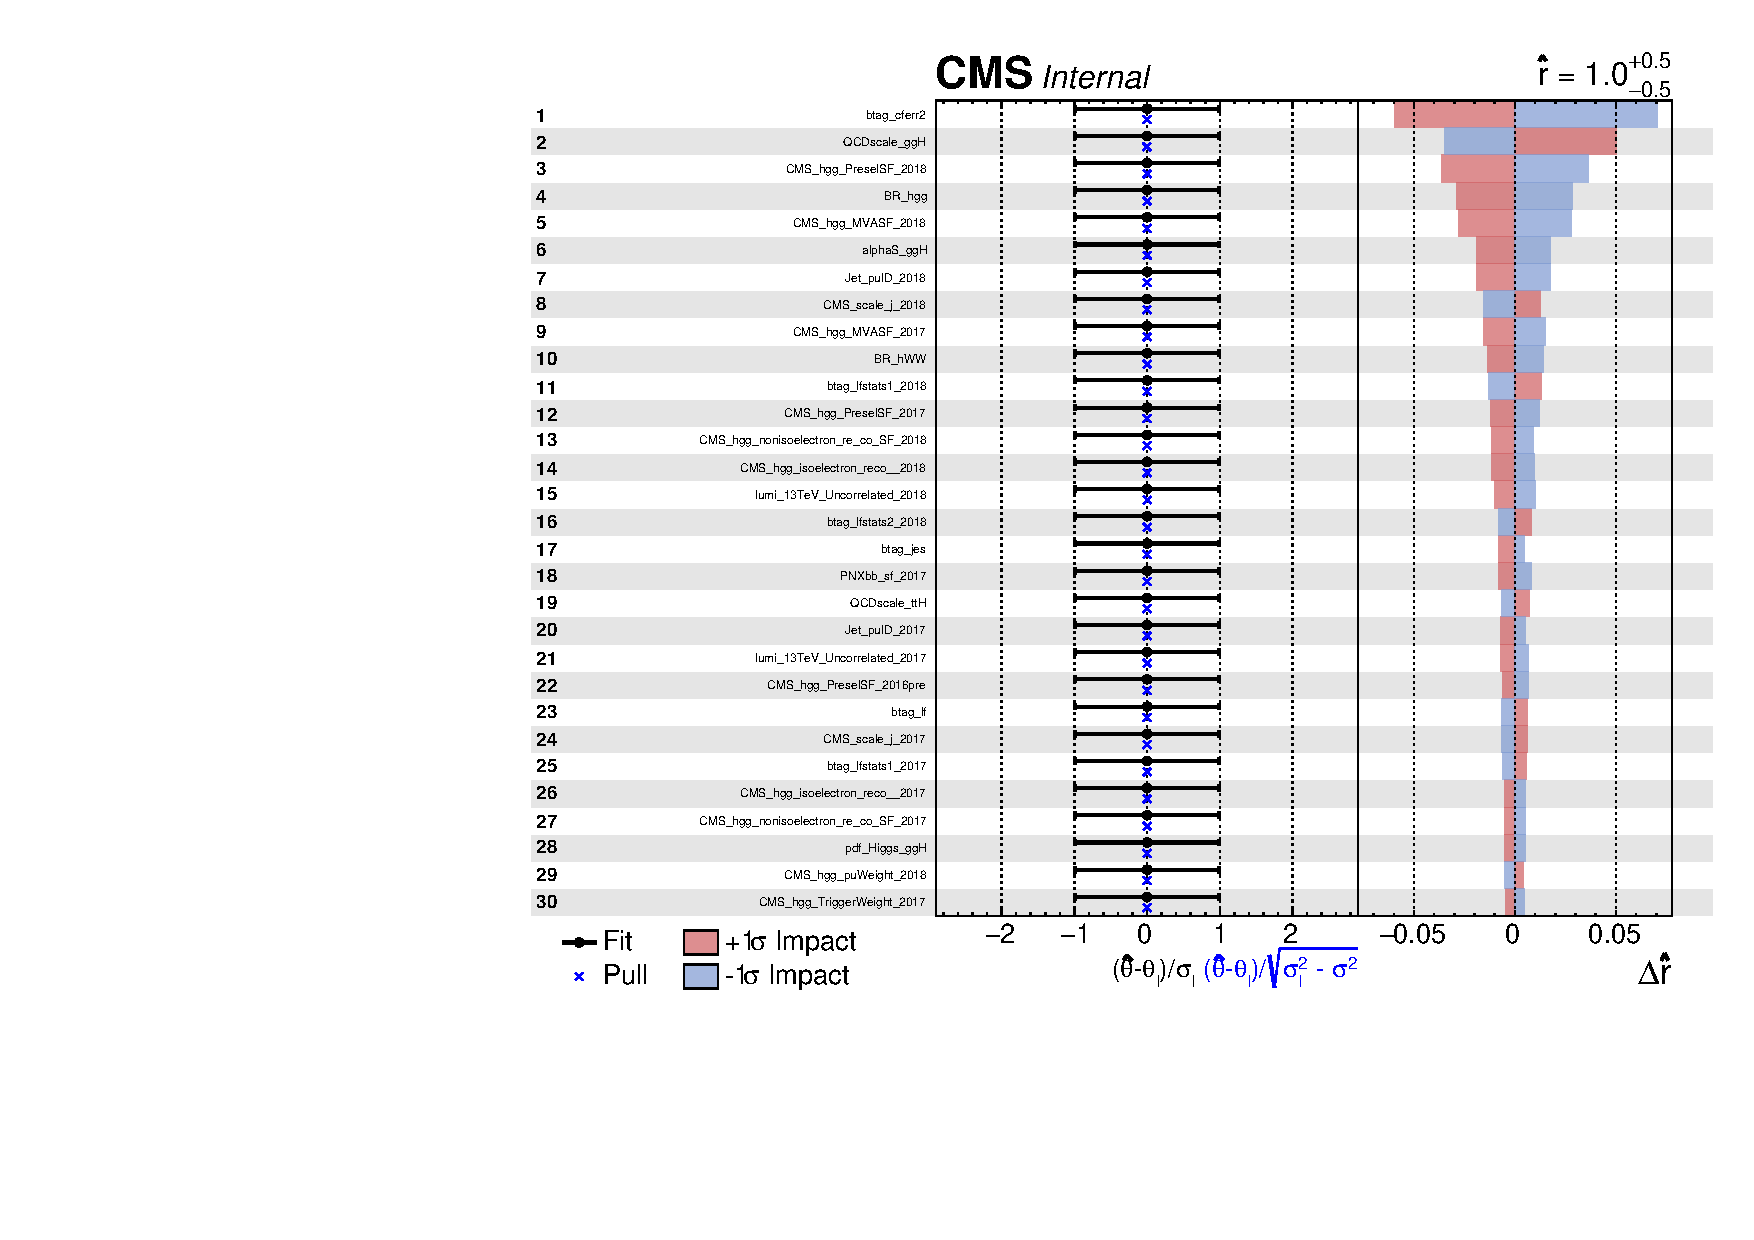
\includegraphics[width=0.9\linewidth]{figures/Impact/MX250_MH125.pdf} \\
  \end{tabular}
\caption{Pulls and impacts of the leading systematic uncertainties for mass point 250 GeV.
}
\label{fig:impacts_0}
\end{figure}

\begin{figure}[hbt!]
  \centering
  \begin{tabular}{c}
      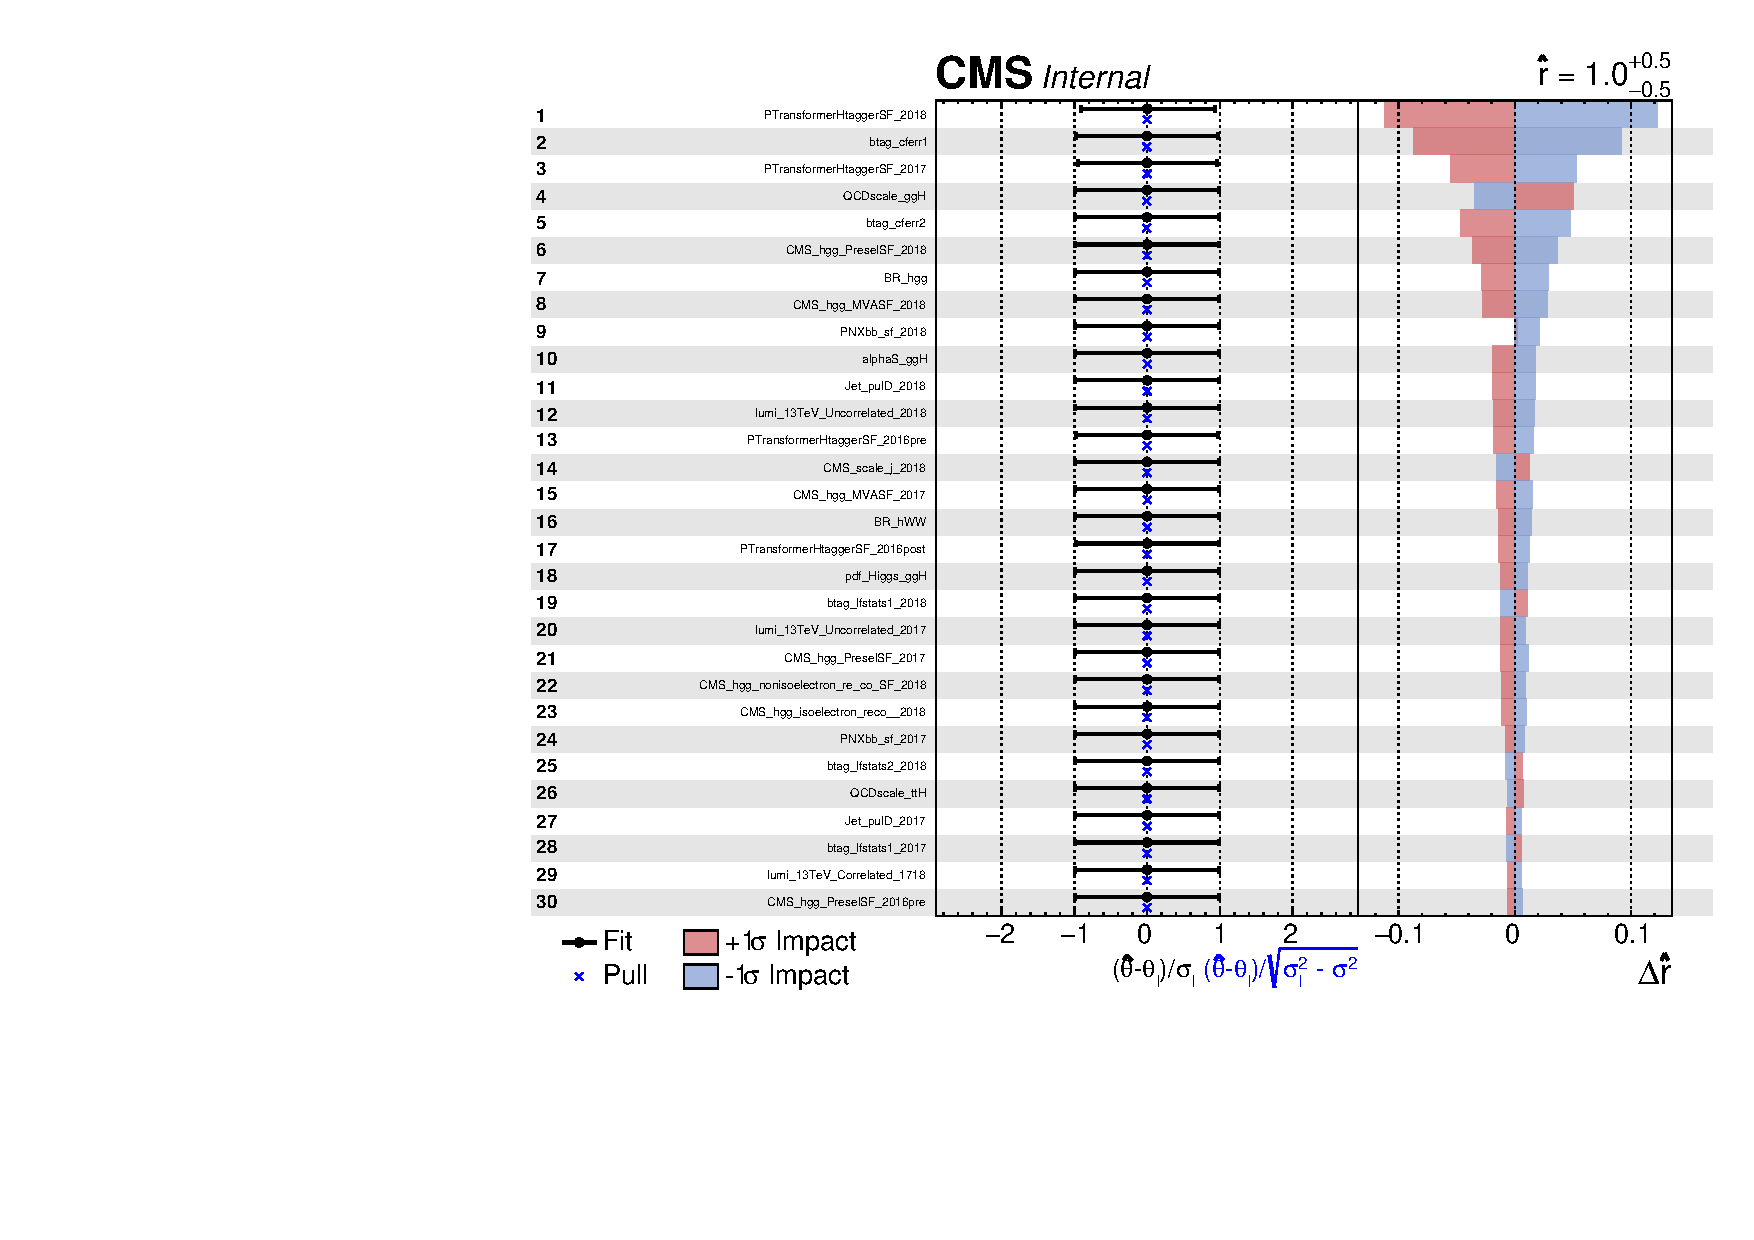
\includegraphics[width=0.9\linewidth]{figures/Impact/MX500_MH125.pdf} \\
  \end{tabular}
\caption{Pulls and impacts of the leading systematic uncertainties for mass point 500 GeV.
}
\label{fig:impacts_1}
\end{figure}


\begin{figure}[hbt!]
    \centering
    \begin{tabular}{c}
        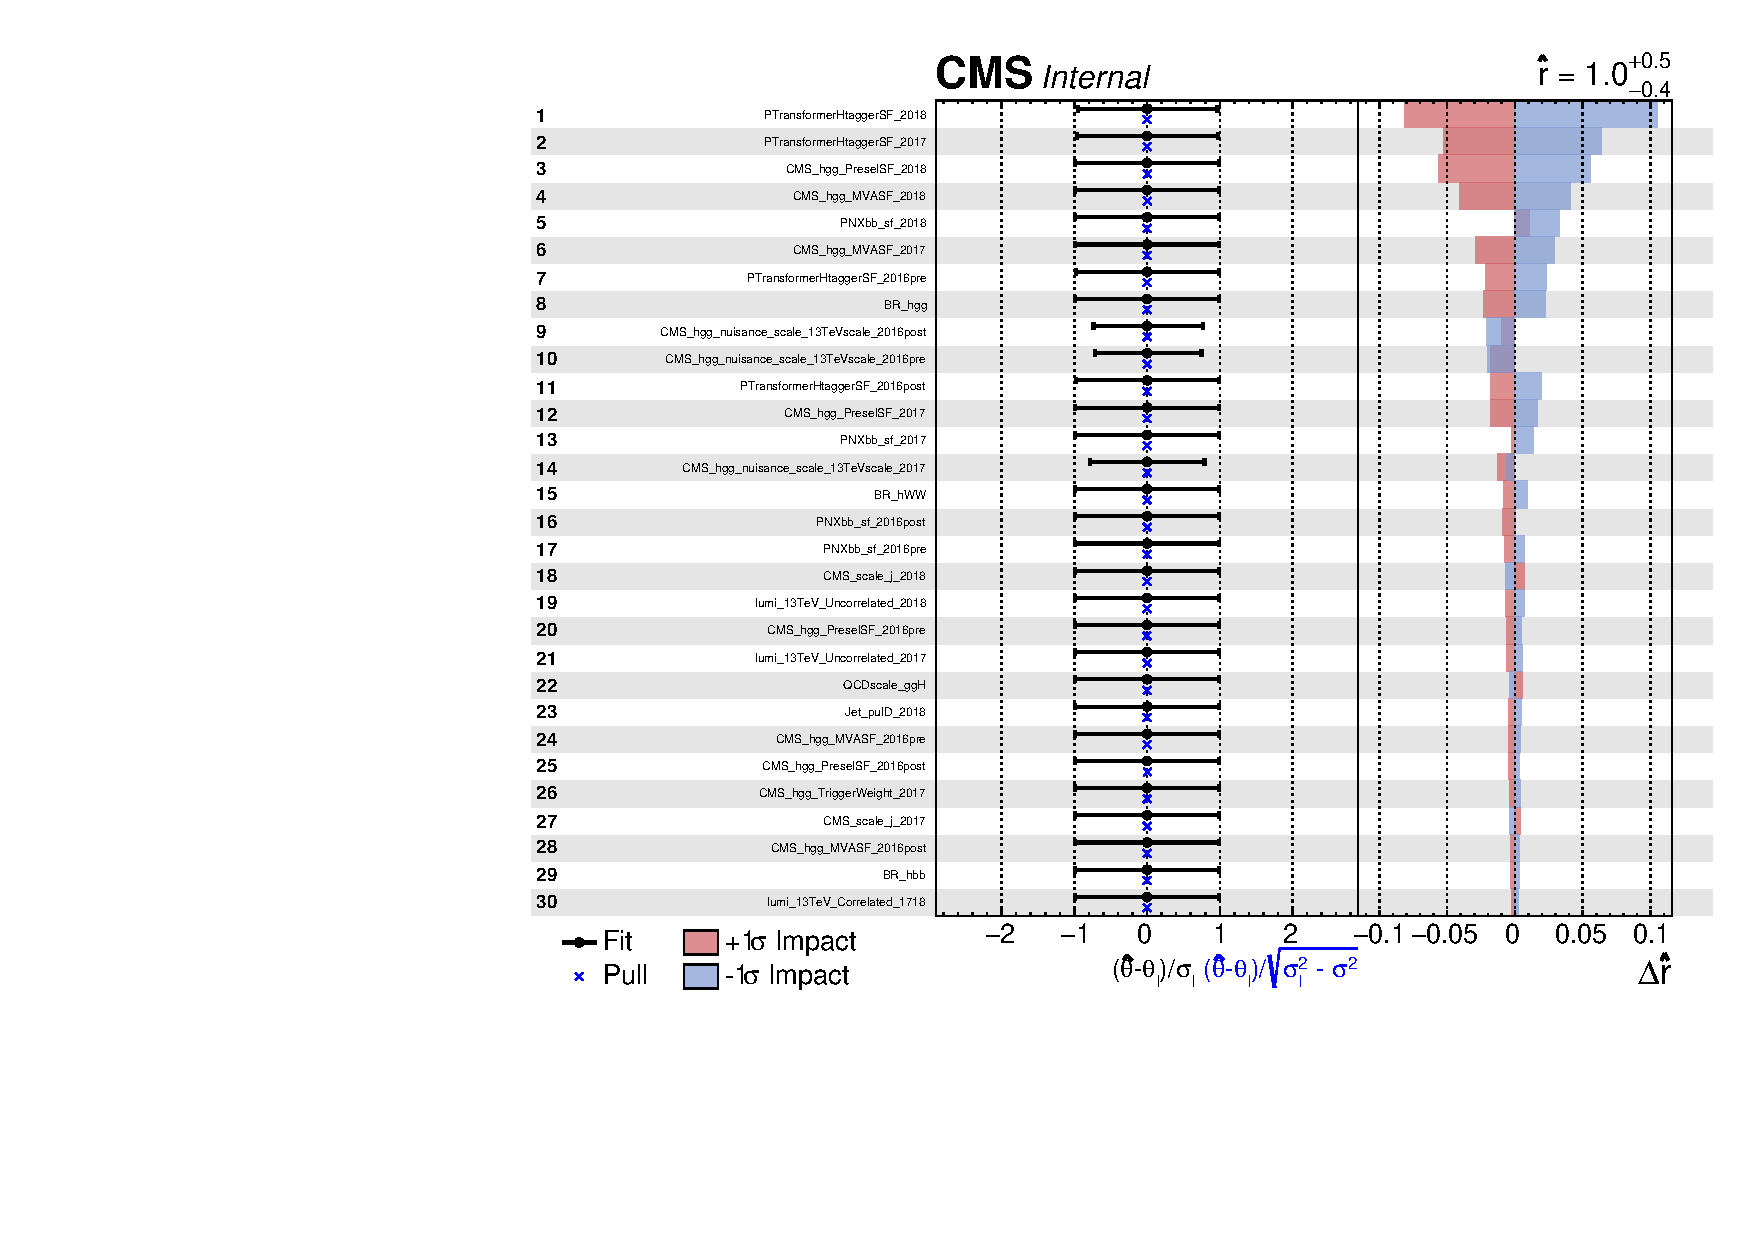
\includegraphics[width=0.9\linewidth]{figures/Impact/MX3000_MH125.pdf} \\
    \end{tabular}
  \caption{Pulls and impacts of the leading systematic uncertainties for mass point 3000 GeV.
  }
  \label{fig:impacts_2}
\end{figure}


\section{Signal and Background Modelling}
\label{sec:signal_background_modelling}

The extraction of the \(X \to HH \to WW\gamma\gamma\) signal is performed using the same methodology as the Higgs boson analysis in the \(H \to \gamma\gamma\) channel~\cite{CMS:2020xrn}. This involves precise modelling of the signal shape using simulated samples and the background shape using data-driven techniques.

\subsection{Signal Modelling}
The signal shape is parameterized based on Monte Carlo (MC) simulations, with the diphoton invariant mass \(m_{\gamma\gamma}\) as the primary observable.

\begin{itemize}
    \item \textbf{Signal Simulation:}
    \begin{itemize}
        \item Signal samples are generated at leading order (LO) using \textsc{MadGraph5\_aMC@NLO} for the gluon-gluon fusion process \(gg \to X\).
        \item Subsequent parton showering and hadronization are performed with \textsc{Pythia8}, and detector effects are simulated using the CMS \textsc{Geant4}-based framework.
        \item Simulated samples are produced for resonance masses \(m_X\) ranging from 250~GeV to 3000~GeV.
    \end{itemize}

    \item \textbf{Signal Shape:}
    \begin{itemize}
        \item The diphoton mass distribution for the signal is modelled using a double-sided Crystal Ball (CB) function, defined as:
        \[
        f_{\text{CB}}(x) =
        \begin{cases}
            A \exp\left(-\frac{(x-\mu)^2}{2\sigma^2}\right), & \text{for } |x-\mu| \leq \alpha\sigma, \\
            B \left(\frac{n}{\alpha} - \frac{n}{\alpha - (x-\mu)/\sigma} \right)^{-n}, & \text{for } x-\mu > \alpha\sigma,
        \end{cases}
        \]
        where \(\mu\) is the mean, \(\sigma\) is the width, and \(\alpha\), \(n\) define the tail parameters.
        \item The parameters of the Crystal Ball function are extracted from fits to the MC simulation in each analysis category (boosted and resolved).
        \item The normalization of the signal is determined from the integrated luminosity and the predicted cross section for \(X \to HH \to WW\gamma\gamma\).
    \end{itemize}

    \item \textbf{Signal Categories:}
    The analysis is divided into multiple categories to maximize sensitivity:
    \begin{itemize}
        \item \textbf{Boosted:} Events where the \(W\)-boson decay products are merged into single large-radius jets.
        \item \textbf{Resolved:} Events where the \(W\)-boson decay products are reconstructed as separate small-radius jets.
        \item \textbf{Semi-leptonic and fully hadronic:} These subcategories depend on the final-state reconstruction of leptons or jets.
    \end{itemize}
\end{itemize}

\subsection{Background Modelling}
The dominant background arises from SM non-resonant diphoton production, with additional contributions from single Higgs production and fake photon processes. The background is modelled using the following approaches:

\begin{enumerate}
    \item \textbf{Non-Resonant Diphoton Background:}
    \begin{itemize}
        \item The continuum diphoton background is modelled directly from data using a smooth analytic function. This function is chosen based on its ability to fit the diphoton invariant mass sidebands while avoiding bias in the signal region.
        \item A range of functional forms, such as exponentials, power laws, or Bernstein polynomials, is tested. The optimal choice is selected using the Fisher F-test and evaluated for bias using pseudo-experiments.
        \item The background shape parameters are determined from fits to the \(m_{\gamma\gamma}\) sideband regions (\(100 < m_{\gamma\gamma} < 120\)~GeV and \(130 < m_{\gamma\gamma} < 180\)~GeV).
    \end{itemize}

    \item \textbf{Resonant Backgrounds:}
    \begin{itemize}
        \item Single Higgs production (\(ggH\), VBF, \(VH\)) with \(H \to \gamma\gamma\) is a subdominant but irreducible background. It is modelled using MC simulation normalized to the theoretical cross sections.
        \item Other rare processes such as \(t\bar{t}\gamma\gamma\), \(W\gamma\gamma\), and \(Z\gamma\gamma\) are also estimated from MC samples.
    \end{itemize}

    \item \textbf{Fake Photon Background:}
    \begin{itemize}
        \item Events where jets or electrons are misidentified as photons are estimated using a data-driven method based on the photon ID MVA sideband technique (Section~\ref{sec:data_driven_bkg}).
        \item The contribution of fake photons is validated in control regions enriched with QCD multijet events.
    \end{itemize}
\end{enumerate}

\subsection{Systematic Uncertainties}
The systematic uncertainties affecting the signal and background modelling include:
\begin{itemize}
    \item \textbf{Signal Modelling:}
    \begin{itemize}
        \item Uncertainty in the Crystal Ball function parameters.
        \item Theoretical uncertainties in the signal cross section due to renormalization and factorization scales.
    \end{itemize}
    \item \textbf{Background Modelling:}
    \begin{itemize}
        \item Uncertainties in the choice of the analytic function for the non-resonant background.
        \item Statistical uncertainties in the fits to sideband data.
    \end{itemize}
    \item \textbf{Experimental Uncertainties:}
    \begin{itemize}
        \item Photon energy scale and resolution uncertainties.
        \item Jet energy scale (JES) and jet energy resolution (JER) uncertainties.
        \item Integrated luminosity uncertainty of 1.6\%.
    \end{itemize}
\end{itemize}

\subsection{Result Extraction}
The signal extraction is performed using an unbinned maximum likelihood fit to the diphoton invariant mass spectrum \(m_{\gamma\gamma}\) in each analysis category. The signal and background components are parameterized as:
\[
f_{\text{total}}(m_{\gamma\gamma}) = N_{\text{sig}} f_{\text{sig}}(m_{\gamma\gamma}) + N_{\text{bkg}} f_{\text{bkg}}(m_{\gamma\gamma}),
\]
where \(f_{\text{sig}}\) is the signal shape modelled by the Crystal Ball function, and \(f_{\text{bkg}}\) is the smooth analytic function for the non-resonant background.

The parameters \(N_{\text{sig}}\) and \(N_{\text{bkg}}\) are extracted simultaneously through the likelihood fit, with systematic uncertainties incorporated as nuisance parameters.


\section{Signal and background modelling} \label{sec:AnalyticFitting}

In order to model the di-Higgs signal process, and single higgs resonant background processes in the signal region, 115 $< \mgg < $ 135 GeV, simulated events
in each analysis category are combined to construct $\mgg$ shapes. Because the continuum background in the signal region is expected to follow a falling
shape continuous with the data sidebands, data events in the data sidebands are fit to a falling analytic function in order to model the continuum background.

\subsection{Di-Higgs signal}
\label{sec:SignalFitting}

Signal shapes for the invariant mass distribution of the diphoton candidate are derived for all analysis categories using simulated events.

Signal models are formed by an analytic fit of a sum of 1-5 Gaussians to a binned $\mgg$ distribution, where the chosen number of Gaussians used in the fit is
determined by an F-test. This is done separately for each year (2016, 2017, 2018) and each analysis category.
The fit for the second highest DNN score region FH category is shown
in Fig.  \ref{fig:FHSignalModel} .

\missingfigure[figwidth=0.75\textwidth]{FH signal model in the second most sensitive category}
\label{fig:FHSignalModel}

% \begin{figure}[!htbp]
%   \centering
%   \includegraphics[width=0.75\textwidth,height=7cm]{figures/AnalyticFitting/Signal/smodel_HHWWggTag_FHDNN_1.pdf}
%   \caption{FH signal model in the second most sensitive category}
% \label{fig:FHSignalModel}
% \end{figure}

\subsection{Single Higgs background}

There are expected resonant background processes present in the signal region, $115 < \mgg < 135$ GeV, due to $H\rightarrow\gamma\gamma$ processes, which cannot be modeled with a data-driven
method using data sideband events. These backgrounds are modeled with MC in the same fashion as the $HH\rightarrow WW\gamma\gamma$ signals as described in Sec. \ref{sec:SignalFitting}. The single higgs
processes considered as resonant backgrounds are the gluon-gluon fusion, vector boson fusion, associated production with a vector boson, and associated production with a top quark pair (ttH), where the Higgs boson decays
into two photons. A separate fit is made for each analysis category and production mode. For cases in which there is a very small number of MC statistics, the diphoton shape from
the di-Higgs signal model in the same analysis category is taken and scaled to the single higgs yield in this category, and used to model the single higgs shape in this category.

\subsection{Continuum background}
\label{sec:AnalyticFitting_Background}

A data-driven background model is produced for each category using the data sidebands in the regions $100 < \mgg < 115$ GeV and $135 < \mgg < 180$ GeV.
The aim of this is to model the continuum background.
After the event selections and categorizations described in Sec. \ref{sec:event_selection} are applied, analytic functions are fit to the resulting $\mgg$ distributions in the data sidebands for each category.
These are later combined with their corresponding signal models in order to extract final results.
As with the signal fitting, an F-Test is performed first in order to obtain initial best-fit estimates for backgrounds functions to the data-sidebands, and to determine which functions will be considered.
Bernstein, laurent, exponential, and powerlaw function families are considered as
candidates to fit the data, and F-Tests are performed for each of these. The three data taking years are merged together before the F-test and function fitting is performed.
After determining which functions pass the F-Test, a best fit function is chosen with the envelope method by treating the choice of function as a discrete nuisance parameter.
An uncertainty is then assigned to the chosen fit function based on a combination of the likelihoods of all attempted fit functions. This method is described in
Ref. \cite{Dauncey_2015}.

After obtaining signal models, continuum background models and Single-Higgs models for each final state, a signal plus background fit is performed.
The combination of all categories' signal plus background fits in the range 100 $<$ $\mgg$ $<$ 180 GeV, where each category is weighted by S over S$+$B, is shown in Figure \ref{fig:Run2SplusB}.

\missingfigure[figwidth=0.7\textwidth]{Combined limit}
\label{fig:Run2SplusB}

% \begin{figure}[!htbp]
%   \centering
%   \includegraphics[width=0.7\textwidth,height=8cm]{figures/Results/All_combined_SplusB.pdf}
%  \caption{The observed diphoton mass distribution including the signal plus background fit (red), the Single-Higgs + continuum background fit (blue) and the continuum background (black dashed line),
%  with bands covering the $\pm 1\sigma$ and $\pm 2\sigma$ uncertainties in the fitted background where all analysis categories are combined and weighted by S over S$+$B.}
%   \label{fig:Run2SplusB}
% \end{figure}

\section{Systematic uncertainties} \label{section:Systematics}
This analysis takes into account systematic uncertainties from theoretical and experimental sources. The uncertainties on the signal and on the single Higgs backgrounds are modeled as scale or shape uncertainties. The scale uncertainties affect the yield of the processes and are treated as log-normal uncertainties, while the shape uncertainties are modeled as variations of the \mgg shape of the processes, i.e. the peak position or the width. The systematic uncertainty associated with the data-driven estimate of the continuum background is accounted for via the discrete profiling method. Given the small number of expected signal events compared to the backgrounds, the effect of the systematics uncertainties on the final results is expected to be small compared to the statistical ones. In case a systematic uncertainty affects processes in different channels, it is considered fully correlated across those channels. The following sources of systematic uncertainties are considered:

\begin{enumerate}

  \item \textbf{Theoretical uncertainties on the HH cross section}: The combined uncertainty on the QCD scale and on the top mass is taken into account, considering also its dependence from the value of $\kappa_{\lambda}$. For the SM signal this uncertainty amounts to $-23/+6\% $. The combined uncertainty on the PDF modeling and on the strong coupling constant is also considered with a value of $3\% $ \cite{Grazzini:2018bsd}.

  \item \textbf{Theoretical uncertainties on the single Higgs cross sections}: Process-dependent uncertainties related to the QCD scale, the PDF modeling, and the strong coupling constant are taken into account for the ggH, ttH, VBF H, and VH processes.

  \item \textbf{Theoretical uncertainties on the Higgs boson branching ratios}: Such uncertainties are considered for both the single and the double Higgs processes. The considered uncertainties on the $H\rightarrow\gamma\gamma$, $H\rightarrow VV$, and $H\rightarrow bb$ branching ratios are approximately $2\% $, $1.5\% $, and $1.2\% $, respectively.

  \item \textbf{Integrated luminosity}: A scale uncertainty is defined according to the luminosity measurements performed by the CMS experiment ~\cite{CMS-LUM-17-003,CMS-PAS-LUM-17-004,CMS-PAS-LUM-18-002}.

  \item \textbf{Trigger}: The trigger efficiency is measured from data with a tag and probe procedure using $Z \rightarrow ee$ events. The related uncertainty is uncorrelated between the three data taking years. An additional considered source of uncertainty is related to inefficiencies of the ECAL L1 trigger at $|\eta|>2$ experienced during 2016 and 2017. This is modeled as a purely rate-changing uncertainty.

%  \item \textbf{Pile-up reweigthing}: The distribution of the simultaneous number of interactions in the Monte Carlo simulation is corrected to match the one observed in the data through an event reweight procedure. The uncertainty on the number of pile-up events is estimated by varying the proton-proton inelastic cross section, 69.2 mb, within $\pm$ 4.6\%. This is modeled as a scale uncertainty uncorrelated between the three data taking years.

  \item \textbf{Electron and muon reconstruction, identification and isolation efficiency}: These efficiencies are evaluated in data and simulation with tag-and-probe techniques using Drell-Yan events \cite{Khachatryan:2015hwa, Sirunyan:2018fpa}. Scale factors are derived and applied to the simulated events to improve the agreement of the efficiencies between simulation and data. The related uncertainty is purely rate-changing and uncorrelated between the three data taking years.

  \item \textbf{Photon identification}: The efficiency of the pre-selection on the photon identification MVA score is estimated in data and simulation with a tag-and-probe technique using Drell-Yan events. Scale factors are applied to correct for the difference between the data and the simulation. The related uncertainty is purely rate-changing  and uncorrelated between the three data taking years.

%  \item \textbf{Electron energy scale and resolution}: Corrections for the energy scale observed in the data are applied to match the simulated one, and for the energy resolution observed in the simulation to match the one observed in the data. The systematic uncertainty on the electron energy scale and resolution is taken considering the POG provided resolution error and the uncertainty on the electron $p_T$. This uncertainty is uncorrelated between the three data taking years.

  \item \textbf{Photon shower shape}: Corrections for the imperfect modeling of the photon shower shape (and isolation) variables in simulation are applied to improve the agreement with the data. The impact of this uncertainty is estimated from the difference of the photon energy scale before and after the correction. This is modeled as a shape uncertainty which is correlated between the three years of the data taking.

  \item \textbf{Photon energy scale and resolution}: Corrections for the difference of the photon energy scale and resolution between data and simulation are derived using $Z \rightarrow ee$ events, with electron-photon differences accounted for as a systematic uncertainty. This uncertainty is uncorrelated between the three years of the data taking.

% Not sure if we apply this. Check: https://github.com/atishelmanch/flashgg/blob/HHWWgg_dev/Taggers/interface/HHWWggTagProducer.h
%   \item \textbf{Di-photons vertex identification efficiency}: Scale factors are computed to account for the difference between data and simulation in number of events for which the correct vertex has been selected.

  %https://twiki.cern.ch/twiki/bin/view/CMS/JECUncertaintySources#Recommendation_for_analysis
  \item \textbf{Jet energy scale and resolution}: Corrections for the differences in the measured jet energies between data and simulation are applied \cite{Khachatryan:2016kdb}. The impact of the corresponding uncertainties on the signal yield is evaluated by varying the corrected jets four-momentum within their respective per-jet uncertainties and propagating the effect to the final result. Several sources of uncertainty are considered, each with a specific level of correlation among the three years of data taking.

  \item \textbf{B-tagging}: The difference in the b-tagging score distribution between data and simulation is corrected for with a reweight of the simulated events dependent on the jet $p_T$, $|\eta|$, and flavor \cite{Sirunyan:2017ezt}. The corresponding uncertainty is purely rate-changing and uncorrelated between the three years of data taking.

%   \item \textbf{b-tagging scale factors}: Applied to each jet as a function of jet $p_T$ and $|\eta|$ in order to account for the efficiency difference in b-tagging and misidentification
%         between data and Monte Carlo simulation \cite{Sirunyan:2017ezt}. The systematic effect is estimated by shifting the scale factor up and down by $\sigma$.
%         The \textbf{1a} method \cite{BtaginMethods} is used to predict the correct event yield in data by changing the weight of the selected Monte Carlo events. This uncertainty is uncorrelated between the three
%         data taking years.




\end{enumerate}

The systematic uncertainties due to finite statistics of Monte Carlo samples for the HH signal are neglected.


\section{Summary and Outlook}
This analysis represents the first CMS study of resonant di-Higgs production in the \(WW\gamma\gamma\) channel, covering all possible jet topologies and using advanced machine learning techniques like parameterized neural networks. The results provide significant constraints on BSM scenarios predicting heavy resonances decaying into Higgs boson pairs.

Future plans include:
\begin{itemize}
    \item Extending the analysis to include non-resonant di-Higgs production.
    \item Finalizing results for publication with a target timeline of Moriond 2025.
\end{itemize}
